\documentclass[10pt]{beamer}

\usetheme{metropolis}
\usepackage{appendixnumberbeamer}
\usepackage[utf8]{inputenc}
\usepackage[russian,francais]{babel}
\usepackage{booktabs}
\usepackage[scale=2]{ccicons}

\usepackage{pgfplots}
\usepgfplotslibrary{dateplot}

\usepackage{xspace}
\newcommand{\themename}{\textbf{\textsc{metropolis}}\xspace}
%%\usepackage{polyglossia}
%%    \setdefaultlanguage{french} % main language
%%    \setotherlanguages{russian, hindi, greek, hebrew} % other languages 
%%\graphicspath{{images/}}	% Put all images in this directory. Avoids clutter.
%%\setmainfont{Latin Modern Roman}
%%\setsansfont{Latin Modern Sans}
%%\setmonofont{Latin Modern Mono}
%%\setmainfont[Ligatures=TeX]{Times New Roman}
%%\newfontfamily{\cyrillicfonttt}{Times New Roman}[Script=Cyrillic]

\title{Programmation de Modèles Linguistiques 1, \\ L5SOPRG L3}
\subtitle{Crédits : Karën Fort (pépites pour le TAL)}
%\subtitle{A modern beamer theme}
\date{}
\author{Gaël Lejeune et Caroline Koudoro-Parfait\\  \quad {gael.lejeune@sorbonne-universite.fr\\} \quad {caroline.parfait@sorbonne-universite.fr\\}}
\institute{Observatoire des Textes des Idées et des Corpus - Obtic,\\ Sorbonne Center for Artificial Intelligence - SCAI,\\ Sens Textes Informatiques Histoire - STIH EA 4509, Sorbonne Université}
 \titlegraphic{\hfill
\includegraphics[height=.7cm]{images/sorbonne.png}}
\begin{document}
\maketitle

\begin{frame}{Plan de la présentation}
  \setbeamertemplate{section in toc}[sections numbered]
  \tableofcontents[hideallsubsections]
\end{frame}
\begin{frame}
  \frametitle{Généralités}
  \begin{block}{Organisation du semestre}
 \begin{itemize}
   \item CM + TD le Vendredi de 8h00 à 12h00 (G. Lejeune et C. Koudoro-Parfait)
   \item Contrôle continu + projet + contrôle terminal
  
  \end{itemize}
  \end{block}
\begin{block}{Ressources}
  \begin{itemize}
  \item \href{http://paris-sorbonne.hosted.exlibrisgroup.com/F?func=find-c&ccl_term=idn=ppn199563403&local_base=MAH01}{TAL et Linguistique Informatique 1}, ISTE Ed. (Mohamed Z. Kurdi) 
  \item Speech and Language Processing (Dan Jurafsky), \url{https://web.stanford.edu/~jurafsky/slp3/} 
  \item Helpdesk : mail ou bureau 206/211 à Serpente (sur RDV)
  \end{itemize}
   \end{block}
\end{frame}

\begin{frame}
  \frametitle{Plan du cours}
\tableofcontents

\end{frame}
\section{Introduction}


\begin{frame}
  \frametitle{Contexte : l'accès aux données langagières}
  \begin{block}{}
    \begin{tabular}{cc}
      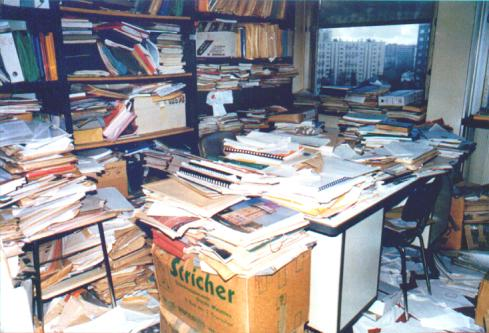
\includegraphics[width=5cm]{images/bordel.png} & 
\includegraphics[width=5cm]{images/seven_library.png}\\
    \end{tabular}
  \end{block}
\end{frame}


\begin{frame}
  \frametitle{Difficulté : des données conçues pour des humains}
  \begin{block}{}
    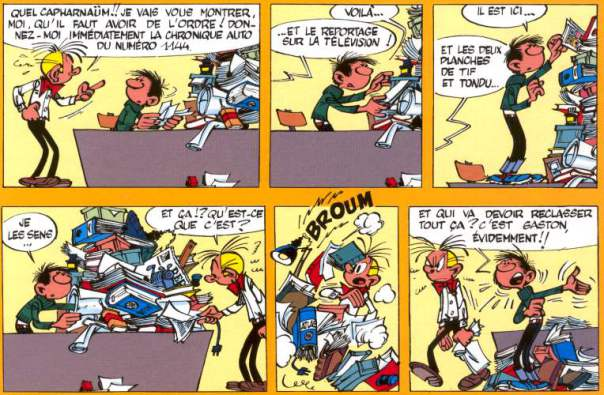
\includegraphics[width=8cm]{images/gaston.jpg}
  \end{block}
\end{frame}

\begin{frame}
  \frametitle{Solution : des données sous-traitées à des machines}
  \begin{block}{}
    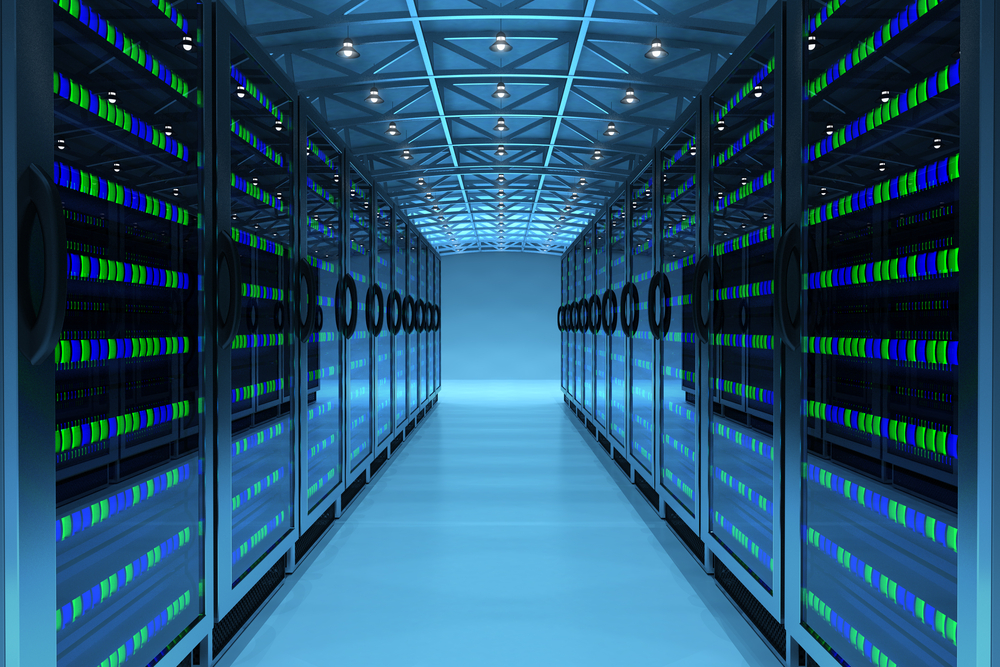
\includegraphics[width=8cm]{images/datacenter1.jpg}
  \end{block}
\end{frame}


\begin{frame}
\frametitle{Objectifs}

\begin{block}{Modéliser la langue}

\begin{itemize}
  \item Observables : le caractère, le phonème, le token
  \item Eco-système : n-grammes, sons, proposition/phrase
  \item Applications : identification de langue, d'auteur, de style; indexation et génération de texte; extraction d'information
\end{itemize}
  Préparation au cours du semestre 6 sur les modèles sémantiques
\end{block}
\end{frame}
%NOTE : Séance 1 (30/09, terminée ici)
\section{Modélisation de la Langue et TAL}
%\subsection{Terminologie}
%\frame{
% \tableofcontents[sectionstyle=show/shaded,subsectionstyle=show/show/hide]
%}

\begin{frame}
\frametitle{Terminologie}
\begin{itemize}
\item Traitement Automatique des Langues
\item Traitement Automatique du Langage Naturel
\pause
\item \textit{Natural Language Processing} 
\item Technologies du Langage (Humain)
\item Sciences de l'information
\item Linguistique Computationnelle
\end{itemize}
\end{frame}

\subsection{Le TAL en 2 minutes}
\begin{frame}
%\frametitle{\foreignlanguage{russian}{Что это?}}
\frametitle{La langue vue par la machine}

\only<1>{
\vspace{5cm}
\begin{center}
   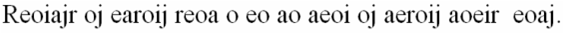
\includegraphics[width=10cm]{images/Picture7.png}
   Langue inconnue
\end{center}
}
\only<2>{
\vspace{5cm}
\begin{center}
   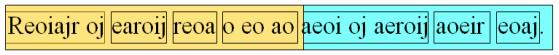
\includegraphics[width=10cm]{images/phrase_tokenized.jpg}
   Découper
\end{center}
}
\only<3>{
\vspace{3.5cm}
\hspace{0.5cm}
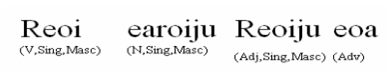
\includegraphics[width=6cm]{images/Picture3.png}
\vspace{0.5cm}
\begin{center}
   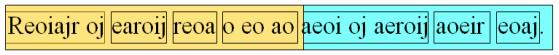
\includegraphics[width=11cm]{images/phrase_tokenized.jpg}
   Etiqueter
\end{center}
}

\only<4>{
\vspace{1cm}
\hspace{0.5cm}
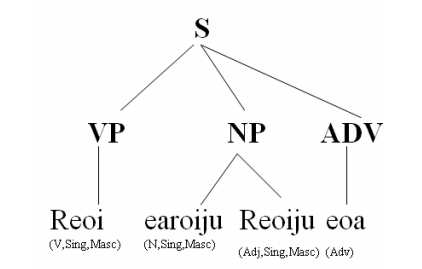
\includegraphics[width=6cm]{images/Picture2.png}
\vspace{0.5cm}
\begin{center}
    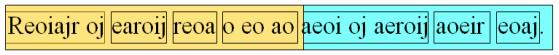
\includegraphics[width=10cm]{images/phrase_tokenized.jpg}
    Reconnaître la structure
\end{center}
}

\only<5>{
\vspace{0.6cm}
\begin{center}
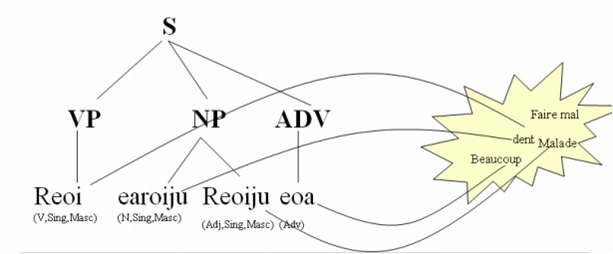
\includegraphics[width=10cm]{images/Picture1.png}
\end{center}
\vspace{0.5cm}
\begin{center}
   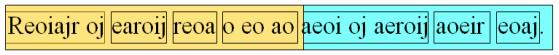
\includegraphics[width=10cm]{images/phrase_tokenized.jpg}
   Évaluer le sens et mettre en contexte
\end{center}
Nécessité d'explicitation (réductionnisme)
}

\end{frame}

\subsection{Le TAL vu par ses applications}

%\begin{frame}
%\frametitle{Applications}
%\only<2>{
%\begin{center}
%   \includegraphics[width=9cm]{images/Picture8.png}
%\end{center}
%}
%\end{frame}

\begin{frame}
\frametitle{Pour quoi faire ?}

\begin{itemize}
\item Traduction automatique
\item Recherche d'information
\item Indexation
\item Traitement d'Emails
\item Veille
\item E-reputation
\item Big Data
\item \ldots
\end{itemize}

\end{frame}

%%\begin{frame}
%%%\frametitle{Marché}
%%
%%\begin{figure}
%%  \begin{center}
%%   \includegraphics[width=9cm]{images/new/Picture9.png}
%%  \caption{Une estimation du poids du marché des industries de la langue (milliards de \$), source \url{http:www.statista.com}}
%%  \end{center}
%%\end{figure}
%%\only<2>{
%%\small{CA Google T1-2013 : \$14 Milliards 
%%\\PIB France 2012 : \$2 800 Milliards}
%%}
%%\end{frame}

%%\begin{frame}
%%\frametitle{Marché par application}
%%
%%\begin{figure}
%%\begin{center}
%%   \includegraphics[width=9cm]{images/new/Picture10.png}
%%\end{center}
%%\caption{Estimation de la demande par sous domaines, source \url{altaplana.com}}
%%\end{figure}
%%\end{frame}

\subsection{Le TAL : définitions}

\begin{frame}
\frametitle{TAL: Modéliser l'activité langagière}

Pour les \textcolor{blue}{chercheurs} :
\begin{itemize}
   \item comprendre comment fonctionne la langue
   \item exemplifier/vérifier des théories
\end{itemize}

\medskip
Pour les \textcolor{blue}{industriels} :
\begin{itemize}
   \item reproduire l'activité langagière
   \item optimiser les performances des systèmes
   \item offrir de nouveaux services
\end{itemize}

\end{frame}

\subsection{Ambiguïté à tous les étages}
\frame{
 \tableofcontents[sectionstyle=show/shaded,subsectionstyle=show/show/hide]
}

\begin{frame}
\frametitle{Le TAL : pas si simple\ldots}
%\begin{block}
\begin{itemize}[<+->]
   \item \textit{La mousse aux fraises est sur la table de l’avocat.} -- polysémie
   \item \textit{L'omelette au lard est parti sans payer !} -- métonymie
   \item \textit{Le bus a renversé un passant}\ldots -- métonymie
   \begin{itemize}
      \item \ldots \textit{je l’ai entendu freiner}. --Contexte
      \item \ldots \textit{je l’ai entendu crier}.
   \end{itemize}
   \item \textit{Le professeur a envoyé l'élève chez le proviseur}\ldots
  \begin{itemize}
      \item \ldots \textit{il faisait trop de bruit}.
     \item \ldots \textit{il était excédé}.
     \item \ldots \textit{il l’avait convoqué}.
\end{itemize}
\end{itemize}

%\end{block}
\bigskip
\only<10>{
$\rightarrow$ \textcolor{blue}{ambiguïtés} pour les systèmes et/ou pour les humains\\
$\rightarrow$ \textcolor{blue}{inférences} difficiles à recenser exhaustivement
}
\end{frame}
\subsection{\'Etapes de traitement}

\begin{frame}
\frametitle{Le découpage en "mots" ou \textit{tokenization}}
\begin{itemize}[<+->]
\item \textit{l’arbre} 
\item \textit{aujourd’hui} 
\end{itemize}
\begin{itemize}[<+->]
\item \textit{plateforme} 
\item \textit{plate-forme} 
\item \textit{dit-il} 
\item \textit{cé-\\sure} 
\pause
\item Va\'blahei\'barvegavinnuverkfærageymsluskúraútidyralyklakippuhringur ("Porte-clés de la chaîne de clé pour la porte extérieure du hangar à outils des agents de la route sur le plateau Va\'blahei\'bi") %ði

\end{itemize}

\end{frame}

\begin{frame}
\frametitle{L'analyse morphologique}
la \textit{porte}

\begin{itemize}[<+->]
\item \textit{porte} +Nom +Fem + Sg
\item \textit{porte} +VT + 1/3P + Sg
\end{itemize}

\end{frame}



\begin{frame}
\frametitle{L'analyse syntaxique}
\textit{ Jean regarde un homme sur la colline avec un télescope.}
\begin{itemize}
\item \textbf{Qui} est sur la colline ?
\item \textbf{Qui} a un télescope ?
\end{itemize}
\begin{itemize}[<+->]
\item Jean regarde [un homme sur la colline avec un télescope]
\item Jean regarde [un homme sur la colline] avec un télescope
\item Jean regarde un homme [sur la colline avec un télescope]
\end{itemize}

\metroset{block=fill}
\pause
\begin{block}{Un défi à l'intuition}
Moi "... Vous avez oublié la pièce jointe..."

Le client mail :
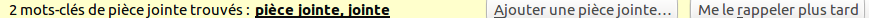
\includegraphics[width=.9\textwidth]{images/PJ_error.png}
\end{block}
\end{frame}


\begin{frame}
\frametitle{L'analyse sémantique}
 \textit{Tous les hommes aiment une femme.}
 \medskip

$\rightarrow$ \textbf{Chaque} homme aime une femme ou 
\\$\rightarrow$  \textbf{tous} les hommes aiment la même femme ?\\
\pause
 \medskip
\textit{The Wayward Pines Trilogy (2012–2014) is a mystery/thriller/science fiction novel series by American author Blake Crouch.}\\
 \medskip
$\rightarrow$ \textbf{Book} = "The Wayward Pines Trilogy", \textbf{Date} ="2012-2014", \textbf{Author}="Blake Crouch"\\
\pause
\medskip
\textit{Jean-Marie Roughol, 47 ans, sort un livre écrit à quatre mains avec le président du Conseil constitutionnel, Jean-Louis Debré}\\
\medskip
$\rightarrow$ \textbf{Book }= "un livre écrit à quatre mains", \textbf{Date }="Today", \textbf{Author}="Jean-Marie Roughol, Président du Conseil Constitutionnel"
\end{frame}

\begin{frame}
  \frametitle{Idiosyncrasie \& compositionnalité}
 Idiosyncrasie : Ox-Beef VS Bœuf
 \pause
  \begin{block}{Différences de représentation et de combinaison}
%% idiosyncrasie_ru-fr.png 
    \begin{table}
  \begin{tabular}{ll}
    {\foreignlanguage{russian}{Русский язык}}& Fran\c cais\\
    \hline
    {\foreignlanguage{russian}{первый}}   &Premier\\
    {\foreignlanguage{russian}{второй}}   &Deuxième\\
    {\foreignlanguage{russian}{этаж}}       &Etage\\
                  ??                      &Premier étage \\
                  \pause
    {\foreignlanguage{russian}{второй этаж}}       &Premier étage\\
    {\foreignlanguage{russian}{первый этаж}} & Rez-de-chaussée\\
{\foreignlanguage{russian}{резь-де-Chaussee}}& Rez-de-chaussée\\
  \end{tabular}
    \end{table}

  \end{block}
\end{frame}


\section{Analyser les caractères }
\begin{frame}
\frametitle{Reconnaître, traiter et structurer les données textuelles}
En pratique pour la machine ?
Les difficultés de programmation algorithmique sur des données textuelles: \\
\begin{itemize}
    \item Comment la machine reconnaît une chaîne de caractère comme un mot ? 

     \item Comment la machine reconnaît des phrases ?
\end{itemize}


\end{frame}


\begin{frame}
\frametitle{Analyse multilingue :  TD1 et 2}

Puis TD3 : Identification de Langue exploitant des propriétés génériques  \\

\begin{itemize}
    \item Pourquoi ?
     \item Usages ?
     \item Méthodes ?
\end{itemize}
\end{frame}





\end{document}
